\documentclass{article}

\usepackage{amsmath, amsthm, amssymb, amsfonts}
\usepackage{thmtools}
\usepackage{graphicx}
\usepackage{setspace}
\usepackage{geometry}
\usepackage{float}
\usepackage{hyperref}
\usepackage[utf8]{inputenc}
\usepackage[english, spanish]{babel}
\usepackage{framed}
\usepackage[dvipsnames]{xcolor}
\usepackage{tcolorbox}
\usepackage{pgfplots}
\usepackage{tikz}
\usepackage{bbm}
\usepackage{enumitem}

\pgfplotsset{compat=1.18}

\colorlet{LightGray}{White!90!Periwinkle}
\colorlet{LightOrange}{Orange!15}
\colorlet{LightGreen}{Green!15}

\newcommand{\HRule}[1]{\rule{\linewidth}{#1}}

\declaretheoremstyle[name=Teorema,]{thmsty}
\declaretheorem[style=thmsty,numberwithin=section]{theorem}
\tcolorboxenvironment{theorem}{colback=LightGray}

\declaretheoremstyle[name=Ejercicio,]{prosty}
\declaretheorem[style=prosty,numberlike=theorem]{exercise}
\tcolorboxenvironment{exercise}{colback=LightOrange}

\declaretheoremstyle[name=Demostración,]{prcpsty}
\declaretheorem[style=prcpsty,numberlike=theorem]{proofs}
\tcolorboxenvironment{proofs}{colback=LightGreen}

\declaretheoremstyle[name={..}, numbered=no,]{prcpsty_nonum}
\declaretheorem[style=prcpsty_nonum,unnumbered]{proofs*} % Unnumbered version
\tcolorboxenvironment{proofs*}{colback=LightGreen}

\pgfmathdeclarefunction{gauss}{2}{\pgfmathparse{1/(#2*sqrt(2*pi))*exp(-((x-#1)^2)/(2*#2^2))}}

\setstretch{1.2}
\geometry{
    textheight=9in,
    textwidth=5.5in,
    top=1in,
    headheight=12pt,
    headsep=25pt,
    footskip=30pt
}

% ------------------------------------------------------------------------------

\begin{document}

% ------------------------------------------------------------------------------
% Cover Page and ToC
% ------------------------------------------------------------------------------

\title{ \normalsize \textsc{}
    \\ [2.0cm]
    \HRule{1.5pt} \\
    \LARGE \textbf{\uppercase{Inferencia Estadística II}
    \HRule{2.0pt} \\ [0.6cm] \LARGE{Tema 4: Técnicas de Bondad de Ajuste} \vspace*{10\baselineskip}}
}

\author{\textbf{Author} \\
    Victor Elvira Fernández, Tomás Ruiz Rojo, Juan Horrillo Crespo \\
    Universidad de Valladolid \\
    \date{\today}}

\maketitle
\newpage

\begin{center}
    \Huge \textbf{AVISO}
\end{center}

Estos apuntes fueron creados de forma voluntaria por un grupo de estudiantes, invirtiendo tiempo, dedicación y esfuerzo para ofrecer información útil a la comunidad. Apreciamos cualquier apoyo que se nos quiera brindar, ya que nos ayuda a continuar con futuros proyectos de este tipo. \\

Si deseas colaborar en esta clase de proyectos puedes contactarnos y unirte o invitarnos a unas ricas patatas 5 salsas por el siguiente enlace:

\vfil

\begin{center}
    \href{https://www.buymeacoffee.com/ApuntesINdat}{\LARGE \textbf{Buy Me a Patatas 5 Salsas}}
    \href{https://www.buymeacoffee.com/ApuntesINdat}{https://www.buymeacoffee.com/ApuntesINdat}
\end{center}

\begin{itemize}
    \item \href{mailto:juan.horrillo22@estudiantes.uva.es}{Mail Juan Horrillo}
    \item \href{mailto:victor.elvira22@estudiantes.uva.es}{Mail Victor Elvira}
    \item \href{mailto:tomas.rojo22@estudiantes.uva.es}{Mail Tomás Rojo}
\end{itemize}

\vfil

Si has colaborado de cualquier forma te agradecemos enormemente.

\tableofcontents
\newpage

% ------------------------------------------------------------------------------

% \section{Examen parcial de los 2 primero temas}

Ejercicio 1  
Un artículo, producto de un tipo de componente mecánico que puede deteriorarse a dos velocidades distintas, depende de factores de fabricación no controlados.  
Se observa que el tiempo de vida ($X$) de cada componente sigue una mezcla de distribuciones exponenciales con las siguientes características:

\begin{itemize}
    \item Con probabilidad \(p\), el componente tiene un tiempo de vida \(X\) que sigue una distribución exponencial con parámetro \(\lambda_1\), lo cual corresponde a componentes con alta resistencia.
    \item Con probabilidad \(1-p\), el componente tiene un tiempo de vida \(X\) que sigue una distribución exponencial con parámetro \(\lambda_2\), lo cual corresponde a componentes con menor resistencia.
\end{itemize}

El fichero \texttt{Tiempos.RData} corresponde a un conjunto de observaciones independientes \(x_1, x_2, \dots \), que representan los tiempos de vida medidos en horas de varios componentes.

\begin{enumerate}
    \item Obtener el EMV y concretar la distribución asintótica del EMV para los parámetros del modelo que subyace para estos datos.  
    \textbf{Nota:} Planteadas las ecuaciones de verosimilitud, utilice la función \texttt{optim} para el cálculo del EMV.

    \[
    f(x, p, \lambda_1, \lambda_2) = p \cdot e^{-\lambda_1 x} + (1-p) \cdot e^{-\lambda_2 x}
    \]

    \[
    L(x, p, \lambda_1, \lambda_2) = \prod_{i=1}^{n} f(x_i, p, \lambda_1, \lambda_2) = \prod_{i=1}^{n} \left( p \cdot e^{-\lambda_1 x_i} + (1-p) \cdot e^{-\lambda_2 x_i} \right)
    \]

    \[
    \log L(x, p, \lambda_1, \lambda_2) = \sum_{i=1}^{n} \log f(x_i, p, \lambda_1, \lambda_2)
    \]

    \[
    \begin{pmatrix}
        \hat{p} \\
        \hat{\lambda}_1 \\
        \hat{\lambda}_2
    \end{pmatrix}
    \sim
    N_3
    \left(
    \begin{pmatrix}
        p \\
        \lambda_1 \\
        \lambda_2
    \end{pmatrix},
    \text{Var}_{\text{EMV}}^{3 \times 3}
    \right)
    \]

    \item Obtener el IC de Wald con confianza aproximada de \(95\%\) para cada parámetro del modelo.

    \[
    \hat{p} \pm \texttt{qnorm}(0.975) \cdot \sqrt{\text{Var}(\hat{p})}
    \]

    \item Obtener el \textit{p-valor} basado en el estadístico de Wald para contrastar la hipótesis \(H_0: \lambda_1 = 0.5\) vs. \(H_a: \lambda_1 \neq 0.5\).

    \[
    W = \frac{(\hat{\lambda}_1 - 0.5)^2}{\text{Var}(\hat{\lambda}_1)} \sim \chi^2_1
    \]

    \item Obtener el \textit{p-valor} basado en el estadístico de RV para contrastar la hipótesis \(H_0: \lambda_1 = 0.5\) vs. \(H_a: \lambda_1 \neq 0.5\).

    \[
    Q_L = 2 \cdot \left[ \log L(\hat{p}, \hat{\lambda}_1, \hat{\lambda}_2, x) - \sup_{p, \lambda_2} \log L(p, \lambda_1 = 0.5, \lambda_2, x) \right] \sim \chi^2_1
    \]

\end{enumerate}

\section{Introducción al test de Bondad de Ajuste}

Hasta ahora los problemas planteados parten de unos datos obtenidos
en un experimento aleatorio del que se conoce el mecanismo con el que se genera (Familia de distribución $P_\theta$).

\textit{\textbf{Definición: }}El Test de Bondad de Ajuste es un test para comprobar si una familia de distribuciones,
 representa correctamente el mecanismo con el que se generaron los datos.

Planteamiento:

$X_1,\dots,X_n$ con funcion de distribución F. Si $F_0$ es una función de distribución conocida, (por ejemplo, una Poisson con $\lambda=3$), el problema se reduce a:

$$H_0: F=F_0 \quad H_1: F \neq F_0$$
$F_0$ está completamente especificada, por lo que es una hipótesis simple.

La hipótesis nula es compuesta si $F_0$ depende de parámetros desconocidos, por ejemplo, una P($\lambda$)

%Posible section: H_0 simple.
Empezamos con el caso de $H_0$ simple. Existen dos tipos de Test de Bondad de Ajuste si $F_0$ es una función de  distribución conocida.
\begin{enumerate}
    \item $F_0$ discreta: Se comparan las frecuencias observadas con las esperadas bajo $H_0$ (Test $\chi^2$). También se puede hacer si $F_0$ es continua agrupando, pero hay tests más potentes para esos casos.
    \item $F_0$ continua: Comparamos la funcion de distribución empírica con la teórica.
\end{enumerate}

\subsection{Test Chi-Cuadrado de Bondad de Ajuste} 

Sea $X_1,\dots,X_n$ con distribución F discreta:
\[
\begin{matrix}
    C_1 \to P_1\\
    \dots \\
    C_k \to P_k
\end{matrix}
\quad
p_j \geq 0,
\quad \sum_{j=1}^{n} p_j=1
\]

Caso en el que $F_0$ completamente especificada bajo $H_0$:

\[
H_0: p=p^0 \quad p=(p_1,\dots,p_k)'
\]
\[
H_1: p \neq p^0 \quad p^0=(p_1^0,\dots,p_k^0)'
\]

Este problema ya lo sabemos resolver: es un contraste para el parámetro p de una distribución multinomial.

Frecuencia observada en $C_j: f_j=\sum_{i=1}^{n} \mathbbm{1}_{(x_i=c_j)}, \quad j=1,\dots,k \quad \sum_{j=1}^{k} f_j=n$

Frecuencia esperada bajo $H_0$ en $C_j$:
\[
e_j=n \cdot P_0(x=c_j)=n \cdot p_j^0
\]
\newpage
\textbf{Ejemplo:}

\[
P(X = x) = 
\left\{
    \begin{matrix}
        \frac{1}{3} & \text{si } x = 0 \\[0.5em]
        \frac{1}{3} & \text{si } x = 1 \\[0.5em]
        \frac{1}{3} & \text{si } x = 2
    \end{matrix}
\right.
\]


\[
H_0:\quad p_1=\frac{1}{3} \quad p_2=\frac{1}{3} \quad p_3=\frac{1}{3}
\]

Tomando una muestra de n=10. Me salen 7 ceros, 2 unos y 1 dos.
A simple vista no parece que siga esa distribución. Usaremos un estadístico para medir lo diferente que es de nuestra distribución.

Lo que esperabamos obtener es:
\[
\begin{matrix}
    e_1=3,33\\
    e_2=3,33\\
    e_3=3,33
\end{matrix}
\]

El test $\chi^2$ de ajuste proporciona unas bases probabilisticas para decidir si las diferencias son suficientemente grandes para que no hayan ocurrido por azar.

El estadístico se define como:

\[
\chi^2=\sum_{j=1}^{k} \frac{(f_j-e_j)^2}{e_j}
\]

Este estadístico es lo que se conoce como distancia $\chi^2$ entre $f_j$ y $e_j$.

Valores grandes en $\chi^2$, frecuencias observadas y esperadas muy diferentes. 
Fijado $\alpha$:
 \begin{itemize}
    \item  Región critica: ($\chi^2 > C_\alpha$)
    \item  p-valor: $p_0(\chi^2>X_{obs})=p_0(\chi^2>t_{obs})$
 \end{itemize}

 Necesitamos conocer la distribución del estadístico bajo $H_0$.
 Se puede conocer de forma exacta aunque es muy complejo. Nos interesará la distribución asintótica para n grande.

 \textbf{Resultado:}
 \[
 \lim_{n \to \infty} P_0(\chi^2 \leq Z)=P(\chi^2_{k-1} \leq Z)
 \]

La distribución asintótica del estadístico $\chi^2$ bajo $H_0$ es $\chi^2_{k-1}$ g'.



Falla el proofs
\begin{proof}
Ya hemos visto que en este contexto \( F_0 \) es una distribución multinomial. 
Vamos a ver que el estadístico \( T \) bajo \( H_0 \) para el modelo multinomial con \( k-1 \) parámetros libres es asintóticamente equivalente al estadístico \( \chi^2_1 \).

Estadístico RV para:

\[
H_0: F = F_0
\]
\[
H_1: F \neq F_0
\]
\newpage
Recordemos:

\[
L(p, x) = \prod_{j=1}^{k} p_j^{f_j} \quad \implies \quad \log L(p, x) = \sum_{j=1}^{k} f_j \log p_j
\]

El estadístico es:

\[
T = 2 \left[\log L(\hat{p}, x) - \log L(p_0, x)\right] = 2 \left[ \sum_{j=1}^{k} f_j \log \hat{p_j} - \sum_{j=1}^{k} f_j \log p_j^0 \right] 
\]\[= -2 \sum_{j=1}^{k} \left( \log p_j^0 - \log \hat{p_j} \right)
\]

Aproximamos \( \log p_j^0 \) por un desarrollo de Taylor en torno a \( \log \hat{p_j} \):

\[
\log p_j^0 \approx \log \hat{p_j} + (p_j^0 - \hat{p_j}) \frac{1}{\hat{p_j}} - \frac{(p_j^0 - \hat{p_j})^2}{2 \cdot \hat{p_j}^2}+ \dots
\]
\[
\to \log p_j^0- \log \hat{p_j}\thickapprox (p^0_j-\hat{p_j}) \frac{1}{\hat{p_j}}- \frac{(p^0_j-\hat{p_j})^2}{2}\frac{1}{\hat{p_j^2}}
\]
Sabiendo que $\hat{p_j}=\frac{f_j}{n}$
\[
=\left(p_j^0-\frac{f_j}{n}\right) \cdot \frac{n}{f_j} - \frac{\left(p_j^0-\frac{f_j}{n}\right)^2}{2}\cdot \left(\frac{n}{f_j}\right)^2 \xrightarrow{c.s.} 0
\]

Esto converge a 0, ya que, por la Ley de los Grandes Números (LGN), \( \frac{F_j}{n} \) es un estimador consistente de \( p_j \):

\[
\lim_{n \to \infty} P \left( \left| \frac{F_j}{n} - p_j \right| > \varepsilon \right) = 0 \quad \forall \varepsilon>0
\]

Por lo tanto, el estadístico T queda:

\[
T = -2 \sum_{j=1}^{k} \left( n \cdot p_j^0 - f_j \right) + \frac{\sum_{j=1}^{k} (f_j - n \cdot p_j^0)^2}{f_j}
\]

\end{proof}


%Falla el proofs

El text $\chi^2$ y el TRV son asintóticamente equivalentes y como TRV converge a $\chi^2_{k-1}$, el estadístico $\chi^2$ también.
Fijado un $\alpha$.
\begin{itemize}
    \item Región critica: $P_0(\chi^2 \geq C_\alpha) \quad C_\alpha=qchisq(1-\alpha,k-1)$
    \item p-valor: $P_0(\chi^2 \geq t_{obs})=1-qchisq(t_{obs},k-1)$
\end{itemize}

Nota:

Esta aproximación es válida para frecuencias mayores o iguales a 5

\textbf{Ejercicio 1:} Script R

\textbf{Ejercicio 4:} En una fábrica con 220 empleados, el número de trabajadores que tuvieron accidentes se recoge en latabla siguiente:
\[
\begin{matrix}
    \text{Nº accidentes} & 0& 1& 2& 3&  4& 5& 6+\\
    \text{Nº trabajadores}&  181& 9& 4&10&7&4&5
\end{matrix}
\]
¿Son estos datos consistentes con la distribución de Poisson con $\lambda=1$?

Tenemos una hipótesis compuesta ya que no conocemos el parámetro de la Poisson.
Si nos dijeran $P(1)$ sería simple.

\[
f(x,1)=\frac{e^{-1}\cdot \lambda^x}{x!}=\frac{e^{-1}}{x!}
\]
\[
p_0^0=e^{-1} ,\quad p_1^0=e^{-1} ,\quad p_2^0=\frac{e^-1}{2} ,\quad \dots,\quad p_6^0=1-\sum_{j=0}^{b}p_j^0
\]
Calculamos las frecuencias esperadas
\[
e_0=220 \cdot e^{-1},\quad e_1=220 \cdot e^{-1}, \quad \dots
\]
\[
\chi^2=\frac{(181-220 \cdot e^{-1})^2}{220 \cdot e^{-1}}+\dots
\]

Es muy probable que no siga una P(1)

\textbf{Ejercicio 10:} Se lanza una moneda hasta que aparece la primera cara. Este experimento se repite 100 veces. LAs frecuencias observadas del numero de ensayos necesarios hasta que aparece la primera cara son:
\[
\begin{matrix}
    \text{Nº ensayos} & 1& 2& 3& 4&5+\\
    \text{Frecuencia} &40&32&15&7& 6
\end{matrix}
\]

¿Se puede concluir que la moneda es perfecta?

Distribución geométrica:
\[
P_p(X=k)=(1-p)^{k-1}p \quad o \quad P_p(X=k)=(1-p)^{k}p
\]
Probabilidad bajo $H_0$.
\[
p_1^0=\frac{1}{2} \quad p_2^0=\frac{1}{2^2} \quad \dots \quad p_5=1-\sum_{k=1}^{4} p_k
\]

\(H_0\): Los datos provienen de una distribución geométrica \(\left(\frac{1}{2}\right)\).

Según el test, no rechazamos \(H_0\).

Si en realidad los datos vienen de una distribución geométrica \(\left(\frac{1}{3}\right)\),  
¿cuál es la probabilidad de que el test lo detecte?  
¿Y si vienen de una distribución geométrica \((0.52)\)?


 
% \subsection{Distribución del test bajo $H_1$}

Podemos aumentar la potencia sacrificando \(\alpha\) o aumentando el tamaño de la muestra.  
Si queremos asegurar una potencia de, por ejemplo, \(0.8\) o \(0.9\), necesitamos calcular cuánto debe valer \(n\).

Para esto, necesitamos conocer la distribución del test bajo \(H_1\).

Resultado:
\[
\lim_{n \to \infty} P_{\theta_1} (\chi^2_{k-1} \leq t) = P(\chi^2_{k-1}(\delta) \leq t)
\]
Donde \(\delta\) es el parámetro de descentralidad para la \(\chi^2_{k-1}\) descentrada.

\textit{\textbf{Definición:}} La distribución asintótica bajo \(H_1\) del estadístico \(\chi^2\) de prueba de ajuste es una \(\chi^2\) descentrada con \(k-1\) grados de libertad y parámetro de descentralidad \(\delta\).

La demostración no está incluida en este curso. Sin embargo, hacemos algunos comentarios sobre esta definición:

\textbf{Comentarios:} %Los comentarios eran formulajos y no me compilan
\begin{enumerate}
    \item   \begin{itemize}
        \item Si \(X\) es una variable aleatoria tal que \(X \sim N(0,1)\), entonces \(X^2 \sim \chi^2_1\).
        \item Si \(X_1, \dots, X_n\) son v.a.i.i.d. \(N(0,1)\), entonces \(\sum_{i=1}^{n} X_i^2 \sim \chi^2_n\).
        \item Si \(X_1, \dots, X_n\) son v.a.i.i.d. \(N(\mu, \sigma^2)\), entonces 
        \(
        \sum_{i=1}^{n} \left( \frac{X_i}{\sigma} \right)^2 \sim \chi^2_n
        \)
        descentrada con parámetro $\delta$.
    \end{itemize}
    \item Para contrastar 
    \[
    \begin{matrix}
        H_0: p_0 = (p_1^0, \dots, p_k^0) \\
        H_1: p \neq p^0
    \end{matrix}
    \]
    si bajo \(H_1\) la alternativa 
    es \(p = (p_1^1, \dots, p_k^1)\), el test \(\chi^2\) sigue 
    una distribución \(\chi^2_{k-1}(\delta)\), donde \(\delta\) 
    mide la distancia entre los dos vectores:
    \[
    \Delta = \sum_{j=1}^{k} \frac{(p_j^1 - p_j^0)^2}{p_j^0}; \quad \delta = n \cdot \Delta
    \]
    O equivalentemente:
    \[
    \delta = \sum_{j=1}^{k} \frac{\left( n \cdot p_j^1 - n \cdot p_j^0 \right)^2}{n \cdot p_j^0}.
    \]
    \item Existen tablas para $\chi_{k-1}^{2'}(\delta)$ (por ejemplo, las tablas estándar de $\chi^2$ descentrada).
\end{enumerate}



\newpage
\subsubsection*{Ejercicio 11:}  
Durante 60 meses consecutivos se observó la variable aleatoria X="nº de accidentes al mes en un cruce de carreteras". Los resultados fueron:
\[
\begin{matrix}
    X & 0 & 1&2& 3+ \\
    \text{Nº de meses} & 23 & 18 & 12 & 7
\end{matrix}
\]
a) Contrastar la hipótesis de que la distribución de X es geométrica: 
\[
G(\theta);p_\theta(X=x)=\theta \cdot (1- \theta)^x, \quad X=0,1,2,\dots
\]

$H_0: X \sim G(\theta)=$EMV para $X \in \{0,1,2,3+\}$

\[
P_0^0=\theta, \quad P_1^0=\theta \cdot (1-\theta), \quad P_2^0=\theta \cdot (1-\theta)^2, \quad P_3^0=(1-\theta)^3
\]
\[
L(\theta,f)=\prod_{j=1}^{4}[p_j^0]^{f_i}= \theta^{23}\cdot(\theta \cdot (1-\theta))^18 \cdot (\theta \cdot (1-\theta)^2)^12 \cdot ((1-\theta)^3)^7
\]
\[
log L(\theta,f)=53 \log \theta+63 \log (1-\theta)
\]
\[
\frac{d \log(\theta,f)}{d \theta}=\frac{53}{\theta}-\frac{63}{1-\theta} \Longrightarrow \hat{\theta}=\frac{53}{53+63}
\]

Test $\chi^2$:

\[
\hat{\chi^2}=\sum_{j=0}^{3} \frac{(f_j-60\cdot P_l^0(\hat{\theta}))^2}{60 \cdot p_j^0(\hat{\theta})} \sim \chi^2_2
\]

b) Potencia de $H_0:G(0.4) \quad B_n(2,0.6)$
\[
P_1(\chi^2> C_{0.05})=P(\chi_3^2(\delta)>C_{0.05})
\]

\[
S=n \cdot \Delta, \quad \Delta=\sum_{j=0}^{3} \left(\frac{(p_j^0-p_j^1)^2}{p_j^0}\right)
\]

\subsubsection{Test de Kolmogorov-Smirnov}

$X_1,\dots, X_n$ i.i.d. con función de distribución F continua y se quiere contrastar
\[
H_0: F=F_0 \quad H_1: F \neq F_0
\]

El test de Kolmogorov-Smirnov es más potente que el $\chi^2$ en el caso de F continua.
Tenemos:
\begin{itemize}
    \item $F_0 \to $ Función de distribusión bajo $H_0$.
    \item $\hat{F_n} \to$ Función de distribución muestral o empírica.
\end{itemize}
\[
\hat{F_n}(\chi)=\frac{1}{n} \sum_{i=1}^{n} \mathbbm{1}_{(x_i \leq \chi)}, \quad \chi \in \mathrm{R}
\]
\newpage
Tambien se puede definir a partir de los estadísticos de orden:

\[
\hat{F_n}(x)=
\left\{
\begin{array}{ll}
    0, & \text{si } \chi \leq \chi_{(1)}\\
    \frac{i}{n} & \text{si } \chi_{(i)} \leq \chi \leq \chi_{(i+1)}, \quad i=1,\dots,n-1 \\
    1 & \text{si } \chi_{n} \leq \chi
\end{array}
\right.
\]


Propiedades:
\begin{enumerate}
    \item $n\cdot \hat{F_n(\chi)}$ es el total de valores de la muestra menores o iguales a $\chi$ y sigue una distribución B(n,F(x)), $\forall \chi \in \mathbb{R}$
    \item Según el resultado anterior, junto con las propiedades de la distribución binomial, se tiene $\hat{F}$(x) es un estimador consistente de F(x)
    \[
    \lim_{n \to \infty} P(| \hat{F_n}(\chi - F(x)| < \epsilon) \to 0
    \]
    \[
    \text{y es CAN: }\sqrt{n}\cdot(\hat{F_n}(x)-F(x))\backsimeq N(0,F(x)(1-F(x)))
    \]
    \item Por el teorema de Glivenko-Cantelli,$\hat{F_n}(\chi)$ converge uniformemente y casi seguro a F($\chi$).
\end{enumerate}

A medida que n crece, al función escalonada de $\hat{F_n}(\chi)$ con saltos en los valores de los estadísticos de orden $X_{(1)},\dots,X_{(n)}$ aproxima la distribución F(x)'.

Por lo tanto cuando n es grande, la mayor diferencia entee $\hat{F_n}((x))$ y F(x) converge a 0.

Este resultado nos sugiere el estadístico $
D_n=sup_\chi[\hat{F_n}(x)-F(x)]
$ es una medida razonable de la precisión de la estimación.

Estadístico de Kolmogorov-Smirnov de una muestra:
\[
    D_n=sup_\chi|\hat{F_n}(\chi)-F_0(\chi)|
\]
El test rechaza la hipótesis para valores garndes del estadísitico ($D_n>C$).
Como siempre debemos conocer la distribución para obtener el valor crítico.

\section{Introducción al test de Bondad de Ajuste}

Hasta ahora los problemas planteados parten de unos datos obtenidos
en un experimento aleatorio del que se conoce el mecanismo con el que se genera (Familia de distribución $P_\theta$).

\textit{\textbf{Definición: }}El Test de Bondad de Ajuste es un test para comprobar si una familia de distribuciones,
 representa correctamente el mecanismo con el que se generaron los datos.

Planteamiento:

$X_1,\dots,X_n$ con funcion de distribución F. Si $F_0$ es una función de distribución conocida, (por ejemplo, una Poisson con $\lambda=3$), el problema se reduce a:
\[
    H_0: F=F_0 \quad H_1: F \neq F_0
\]
$F_0$ está completamente especificada, por lo que es una hipótesis simple.

La hipótesis nula sería compuesta si $F_0$ depende de parámetros desconocidos, por ejemplo, una P($\lambda$)

Empezaremos con el caso de $H_0$ simple. Existen dos tipos de Test de Bondad de Ajuste si $F_0$ es una función de  distribución conocida.
\begin{enumerate}
    \item $F_0$ discreta: Se comparan las frecuencias observadas con las esperadas bajo $H_0$ (Test $\chi^2$). También se puede hacer si $F_0$ es continua agrupando, pero hay tests más potentes para esos casos.
    \item $F_0$ continua: Comparamos la funcion de distribución empírica con la teórica.
\end{enumerate}

\begin{figure}[h!]
    \centering
    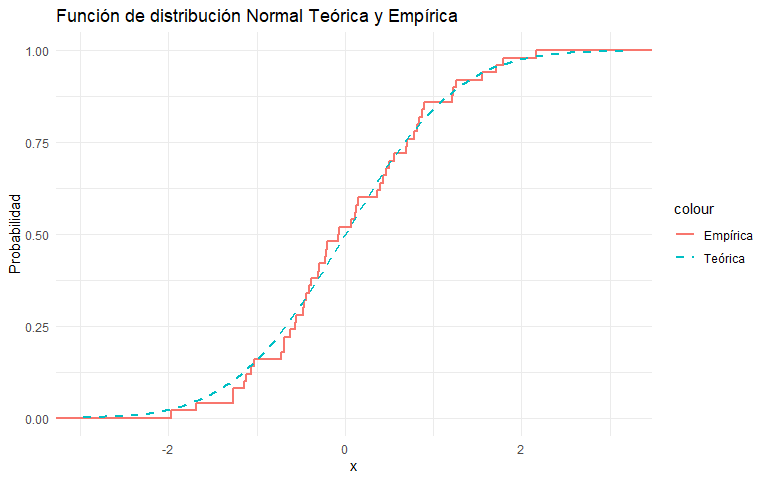
\includegraphics[width=\textwidth]{assets/TeoricaEmpirica.png}
    \caption{Visualización de una distribución teórica y empírica}
    \label{fig:theorical_vs_empirical}
\end{figure}

\subsection{Test Chi-Cuadrado de Bondad de Ajuste}

Sea $X_1,\dots,X_n$ con distribución F discreta:
\[
    \begin{matrix}
        C_1 \to P_1\\
        \dots \\
        C_k \to P_k
    \end{matrix}
    \quad
    p_j \geq 0,
    \quad \sum_{j=1}^{n} p_j=1
\]
Caso en el que $F_0$ completamente especificada bajo $H_0$:
\[
    H_0: p=p^0 \quad p=(p_1,\dots,p_k)'
\]
\[
    H_1: p \neq p^0 \quad p^0=(p_1^0,\dots,p_k^0)'
\]
Este problema ya lo sabemos resolver: es un contraste para el parámetro p de una distribución multinomial.

Frecuencia observada en $C_j: f_j=\sum_{i=1}^{n} \mathbbm{1}_{(x_i=c_j)}, \quad j=1,\dots,k \quad \sum_{j=1}^{k} f_j=n$

Frecuencia esperada bajo $H_0$ en $C_j$:
\[
    e_j=n \cdot P_0(x=c_j)=n \cdot p_j^0
\]

\textbf{Ejemplo:}

Sea una variable aleatoria $X$ cuya función de masa de probabilidad es la siguiente
\[
    P(X = x) = 
    \left\{
        \begin{matrix}
            \frac{1}{3} & \text{si } x = 0 \\[0.5em]
            \frac{1}{3} & \text{si } x = 1 \\[0.5em]
            \frac{1}{3} & \text{si } x = 2
        \end{matrix}
    \right.
\]

Entonces la hipotesis nula para el test será que

\[
    H_0:\quad p_1=\frac{1}{3} \quad p_2=\frac{1}{3} \quad p_3=\frac{1}{3}
\]

Tomando una muestra de n=10 quedan 7 ceros, 2 unos y 1 dos.

\vspace{5mm}

A simple vista no parece que siga esa distribución. Usaremos un estadístico para medir que tan diferente es de nuestra distribución pues lo que esperabamos obtener es:
\[
    \begin{matrix}
        e_1=3,33\\
        e_2=3,33\\
        e_3=3,33
    \end{matrix}
\]
El test $\chi^2$ de ajuste proporciona unas bases probabilisticas para decidir si las diferencias son suficientemente grandes tal que no hayan ocurrido por puro azar. Se define como
\[
    \chi^2=\sum_{j=1}^{k} \frac{(f_j-e_j)^2}{e_j}
\]
Este estadístico es lo que se conoce como distancia $\chi^2$ entre $f_j$ y $e_j$. Para valores grandes en $\chi^2$ implica frecuencias observadas y esperadas muy diferentes. 

\vspace{5mm}

\noindent Fijado $\alpha$:
\begin{itemize}
    \item Región critica: ($\chi^2 > C_\alpha$)
    \item p-valor: $p_0(\chi^2>X_{obs})=p_0(\chi^2>t_{obs})$
\end{itemize}

Necesitamos conocer la distribución del estadístico bajo $H_0$.
Se podría conocer de forma exacta aunque es muy complejo, por ello, nos interesará la distribución asintótica para $n$ grande.

\smallskip

\noindent \textbf{Resultado:}
\[
    \lim_{n \to \infty} P_0(\chi^2 \leq Z)=P(\chi^2_{k-1} \leq Z)
\]
La distribución asintótica del estadístico $\chi^2$ bajo $H_0$ es $\chi^2_{k-1}$ $g'$.

Ya hemos visto que en este contexto $ F_0 $ es una distribución multinomial. 
Vamos a ver que el estadístico $ T $ bajo $ H_0 $ para el modelo multinomial con $ k-1 $ parámetros libres es asintóticamente equivalente al estadístico $ \chi^2_1 $.

\begin{proofs}
    Estadístico RV para:
    \[
        H_0: F = F_0
    \]
    \[
        H_1: F \neq F_0
    \]
    Recordemos:
    \[
        L(p, x) = \prod_{j=1}^{k} p_j^{f_j} \quad \implies \quad \log L(p, x) = \sum_{j=1}^{k} f_j \log p_j
    \]
    El estadístico es:
    \[
        T = 2 \left[\log L(\widehat{p}, x) - \log L(p_0, x)\right] = 2 \left[ \sum_{j=1}^{k} f_j \log \widehat{p_j} - \sum_{j=1}^{k} f_j \log p_j^0 \right] 
    \]
    \[
        = -2 \sum_{j=1}^{k} \left( \log p_j^0 - \log \widehat{p_j} \right)
    \]
    Aproximamos $\log p_j^0$ por un desarrollo de Taylor en torno a $\log \widehat{p_j}$:
    \[
        \log p_j^0 \approx \log \widehat{p_j} + (p_j^0 - \widehat{p_j}) \frac{1}{\widehat{p_j}} - \frac{(p_j^0 - \widehat{p_j})^2}{2 \cdot \widehat{p_j}^2}+ \dots
    \]
    \[
        \to \log p_j^0- \log \widehat{p_j}\thickapprox (p^0_j-\widehat{p_j}) \frac{1}{\widehat{p_j}}- \frac{(p^0_j-\widehat{p_j})^2}{2}\frac{1}{\widehat{p_j^2}}
    \]
\end{proofs}

\newpage

\begin{proofs*}
    Sabiendo que $\widehat{p_j}=\frac{f_j}{n}$
    \[
        =\left(p_j^0-\frac{f_j}{n}\right) \cdot \frac{n}{f_j} - \frac{\left(p_j^0-\frac{f_j}{n}\right)^2}{2}\cdot \left(\frac{n}{f_j}\right)^2 \xrightarrow{c.s.} 0
    \]
    Esto converge a 0, ya que, por la Ley de los Grandes Números (LGN), $\frac{F_j}{n}$ es un estimador consistente de $p_j$:
    \[
        \lim_{n \to \infty} P \left( \left| \frac{F_j}{n} - p_j \right| > \varepsilon \right) = 0 \quad \forall \varepsilon>0
    \]
    Por lo tanto, el estadístico T queda:
    \[
        T = -2 \sum_{j=1}^{k} \left( n \cdot p_j^0 - f_j \right) + \frac{\sum_{j=1}^{k} (f_j - n \cdot p_j^0)^2}{f_j}
    \]
\end{proofs*}

El text $\chi^2$ y el TRV son asintóticamente equivalentes y como TRV converge a $\chi^2_{k-1}$, el estadístico $\chi^2$ también.
Fijado un $\alpha$.
\begin{itemize}
    \item Región critica: $P_0(\chi^2 \geq C_\alpha) \quad C_\alpha=qchisq(1-\alpha,k-1)$
    \item p-valor: $P_0(\chi^2 \geq t_{obs})=1-qchisq(t_{obs},k-1)$
\end{itemize}

\noindent \textit{Nota}:

Esta aproximación es válida para frecuencias mayores o iguales a 5

\vspace{5mm}

\textbf{Ejercicio 1}: Script R

\vspace{5mm}

\textbf{Ejercicio 4}: En una fábrica con 220 empleados, el número de trabajadores que tuvieron accidentes se recoge en latabla siguiente:

\begin{table}[!h]
    \centering
    \begin{tabular}{|c|c|c|c|c|c|c|c|}
        \hline
        {Nº accidentes} & 0 & 1 & 2 & 3 & 4 & 5 & 6+ \\ \hline
        {Nº trabajadores} & 181 & 9 & 4 & 10 & 7 & 4 & 5 \\ \hline
    \end{tabular}
\end{table}

¿Son estos datos consistentes con la distribución de Poisson con $\lambda=1$?

Tenemos una hipótesis compuesta ya que no conocemos el parámetro de la Poisson.
Si nos dijeran $P(1)$ sería simple.

\[
    f(x,1)=\frac{e^{-1}\cdot \lambda^x}{x!}=\frac{e^{-1}}{x!}
\]
\[
    p_0^0=e^{-1} ,\quad p_1^0=e^{-1} ,\quad p_2^0=\frac{e^-1}{2} ,\quad \dots,\quad p_6^0=1-\sum_{j=0}^{b}p_j^0
\]

Calculamos las frecuencias esperadas

\[
    e_0=220 \cdot e^{-1},\quad e_1=220 \cdot e^{-1}, \quad \dots
\]
\[
    \chi^2=\frac{(181-220 \cdot e^{-1})^2}{220 \cdot e^{-1}}+\dots
\]

Por tanto concluimos que es muy probable que no siga una P(1)

\textbf{Ejercicio 10:} Se lanza una moneda hasta que aparece la primera cara. Este experimento se repite 100 veces. LAs frecuencias observadas del numero de ensayos necesarios hasta que aparece la primera cara son:

\begin{table}[!h]
    \centering
    \begin{tabular}{|c|c|c|c|c|c|}
        \hline
        {Nº ensayos} & 1 & 2 & 3 & 4 & 5+ \\ \hline
        {Frecuencia} & 40 & 32 & 15 & 7 & 6 \\ \hline
    \end{tabular}
\end{table}

¿Se puede concluir que la moneda es perfecta?

Distribución geométrica:
\[
    P_p(X=k)=(1-p)^{k-1}p \quad o \quad P_p(X=k)=(1-p)^{k}p
\]
Probabilidad bajo $H_0$.
\[
    p_1^0=\frac{1}{2} \quad p_2^0=\frac{1}{2^2} \quad \dots \quad p_5=1-\sum_{k=1}^{4} p_k
\]

Como $H_0$ es ``Los datos provienen de una distribución geométrica $\left(\frac{1}{2}\right)$''.

Según el test, no rechazamos $H_0$.

Si en realidad los datos vienen de una distribución geométrica $\left(\frac{1}{3}\right)$,  
¿cuál es la probabilidad de que el test lo detecte?  
¿Y si vienen de una distribución geométrica $(0.52)$?

\subsection{Distribución del test bajo $H_1$}

Podemos aumentar la potencia sacrificando $\alpha$ o aumentando el tamaño de la muestra.  
Si queremos asegurar una potencia de, por ejemplo, $0.8$ o $0.9$, necesitamos calcular cuánto debe valer $n$.

Para esto, necesitamos conocer la distribución del test bajo $H_1$.

Resultado:
\[
\lim_{n \to \infty} P_{\theta_1} (\chi^2_{k-1} \leq t) = P(\chi^2_{k-1}(\delta) \leq t)
\]
Donde $\delta$ es el parámetro de descentralidad para la $\chi^2_{k-1}$ descentrada.

\textit{\textbf{Definición:}} La distribución asintótica bajo $H_1$ del estadístico $\chi^2$ de prueba de ajuste es una $\chi^2$ descentrada con $k-1$ grados de libertad y parámetro de descentralidad $\delta$.

La demostración no está incluida en este curso. Sin embargo, hacemos algunos comentarios sobre esta definición:

\textbf{Comentarios:} %Los comentarios eran formulajos y no me compilan
\begin{enumerate}
    \item   \begin{itemize}
        \item Si $X$ es una variable aleatoria tal que $X \sim N(0,1)$, entonces $X^2 \sim \chi^2_1$.
        \item Si $X_1, \dots, X_n$ son v.a.i.i.d. $N(0,1)$, entonces $\sum_{i=1}^{n} X_i^2 \sim \chi^2_n$.
        \item Si $X_1, \dots, X_n$ son v.a.i.i.d. $N(\mu, \sigma^2)$, entonces 
        $
        \sum_{i=1}^{n} \left( \frac{X_i}{\sigma} \right)^2 \sim \chi^2_n
        $
        descentrada con parámetro $\delta$.
    \end{itemize}
    \item Para contrastar 
    \[
    \begin{matrix}
        H_0: p_0 = (p_1^0, \dots, p_k^0) \\
        H_1: p \neq p^0
    \end{matrix}
    \]
    si bajo $H_1$ la alternativa 
    es $p = (p_1^1, \dots, p_k^1)$, el test $\chi^2$ sigue 
    una distribución $\chi^2_{k-1}(\delta)$, donde $\delta$ 
    mide la distancia entre los dos vectores:
    \[
    \Delta = \sum_{j=1}^{k} \frac{(p_j^1 - p_j^0)^2}{p_j^0}; \quad \delta = n \cdot \Delta
    \]
    O equivalentemente:
    \[
    \delta = \sum_{j=1}^{k} \frac{\left( n \cdot p_j^1 - n \cdot p_j^0 \right)^2}{n \cdot p_j^0}.
    \]
    \item Existen tablas para $\chi_{k-1}^{2'}(\delta)$ (por ejemplo, las tablas estándar de $\chi^2$ descentrada).
\end{enumerate}

\subsubsection*{Ejercicio 11:}  
Durante 60 meses consecutivos se observó la variable aleatoria X="nº de accidentes al mes en un cruce de carreteras". Los resultados fueron:

\begin{table}[!h]
    \centering
    \begin{tabular}{|c|c|c|c|c|}
        \hline
        {$X$} & 0 & 1 & 2 & 3+ \\ \hline
        {Nº de meses} & 23 & 18 & 12 & 7 \\ \hline
    \end{tabular}
\end{table}

\begin{enumerate}[label=\alph*)]
    \item Contrastar la hipótesis de que la distribución de X es geométrica:
    \[
        G(\theta);p_\theta(X=x)=\theta \cdot (1- \theta)^x, \quad X=0,1,2,\dots
    \]

    $H_0: X \sim G(\theta)=$EMV para $X \in \{0,1,2,3+\}$

    \[
        P_0^0=\theta, \quad P_1^0=\theta \cdot (1-\theta), \quad P_2^0=\theta \cdot (1-\theta)^2, \quad P_3^0=(1-\theta)^3
    \]
    \[
        L(\theta,f)=\prod_{j=1}^{4}[p_j^0]^{f_i}= \theta^{23}\cdot(\theta \cdot (1-\theta))^18 \cdot (\theta \cdot (1-\theta)^2)^12 \cdot ((1-\theta)^3)^7
    \]
    \[
        log L(\theta,f)=53 \log \theta+63 \log (1-\theta)
    \]
    \[
        \frac{d \log(\theta,f)}{d \theta}=\frac{53}{\theta}-\frac{63}{1-\theta} \Longrightarrow \widehat{\theta}=\frac{53}{53+63}
    \]
    Test $\chi^2$:
    \[
        \widehat{\chi^2}=\sum_{j=0}^{3} \frac{(f_j-60\cdot P_l^0(\widehat{\theta}))^2}{60 \cdot p_j^0(\widehat{\theta})} \sim \chi^2_2
    \]

    \item Potencia de $H_0:G(0.4) \quad B_n(2,0.6)$:
    \[
        P_1(\chi^2> C_{0.05})=P(\chi_3^2(\delta)>C_{0.05})
    \]
    \[
        S=n \cdot \Delta, \quad \Delta=\sum_{j=0}^{3} \left(\frac{(p_j^0-p_j^1)^2}{p_j^0}\right)
    \]
\end{enumerate}

\subsection{Test de Kolmogorov-Smirnov}
\subsubsection{Test de Kolmogorov-Smirnov para hipótesis simples}

$X_1,\dots, X_n$ i.i.d. con función de distribución F continua y se quiere contrastar
\[
    H_0: F=F_0 \quad H_1: F \neq F_0
\]

El test de Kolmogorov-Smirnov es más potente que el $\chi^2$ en el caso de F continua.
Tenemos:
\begin{itemize}
    \item $F_0 \to $ Función de distribución bajo $H_0$.
    \item $\widehat{F_n} \to$ Función de distribución muestral o empírica.
\end{itemize}
\[
    \widehat{F_n}(x)=\frac{1}{n} \sum_{i=1}^{n} \mathbbm{1}_{(x_i \leq x)}, \quad x \in \mathbb{R}
\]
Tambien se puede definir a partir de los estadísticos de orden:

\[
    \widehat{F_n}(x)=
    \left\{
    \begin{array}{ll}
        0, & \text{si} \quad x \leq X_{(1)}\\
        \frac{i}{n} & \text{si} \quad X_{(i)} \leq x \leq X_{(i+1)}, \quad i=1, \dots,n-1 \\
        1 & \text{si} \quad X_n \leq x
    \end{array}
    \right.
\]
\newpage

Propiedades:
\begin{enumerate}
    \item $n\cdot \widehat{F_n}(x)$ es el total de valores de la muestra menores o iguales a $x$ y sigue una distribución $B(n, F(x))$, $\forall x \in \mathbb{R}$
    \item Según el resultado anterior, junto con las propiedades de la distribución binomial, se tiene $\widehat{F}(x)$ es un estimador consistente de $F(x)$
    \[
        \lim_{n \to \infty} P(|\widehat{F_n}(x) - F(x)| < \varepsilon) \to 0
    \]
    \[
        \text{y es CAN: }\sqrt{n}\cdot(\widehat{F_n}(x)-F(x))\backsimeq N(0,F(x)(1-F(x)))
    \]
    \item Por el teorema de Glivenko-Cantelli, $\widehat{F_n}(x)$ converge uniformemente y casi seguro a $F(x)$.
\end{enumerate}

A medida que n crece, al función escalonada de $\widehat{F_n}(x)$ con saltos en los valores de los estadísticos de orden $X_{(1)},\dots,X_{(n)}$ aproxima la distribución $F(x)'$.  % Creo que eso no debería ser prima pero no soy un experto

Por lo tanto cuando n es grande, la mayor diferencia entre $\widehat{F_n}(x)$ y $F(x)$ converge a 0.

Este resultado nos sugiere el estadístico $D_n=sup_x[\widehat{F_n}(x)-F(x)]$ el cual es una medida razonable de la precisión de la estimación.

Llamaremos estadístico de Kolmogorov-Smirnov de una muestra a
\[
    D_n=sup_x|\widehat{F_n}(x)-F_0(x)|
\]
El test rechaza la hipótesis para valores grandes del estadísitico ($D_n>C$).
Como siempre debemos conocer la distribución de $D_n$ para obtener el valor crítico.

\begin{enumerate}
    \item Es importante ver que la máxima diferencia en $|\widehat{F_n}(x)-F_0(x)|$ es la máxima 
    diferencia en los puntos en los que $\widehat{F_n}(x)>F_0(x)$ y la máxima en los punto donde $F_0(x)>\widehat{F_n}(x)$. 
    Así podemos definir los estadísticos Kolmogorov-Smirnov de un lado.
    \[
        \left.\begin{matrix}
                D_n^+=sup_x(\widehat{F_n}(x)-F_0(x)) \\
                D_n^-=sup_x(F_0(x)-\widehat{F_n}(x))
        \end{matrix}\right\}
        D_n=max\{D_n^+,D_n^-\}
    \]
            
    $D_n^+$ y $D_n^-$ son útiles para conocer la distribución.

    \item La distribución de $D_n^+$, $D_n^-$ y $D_n$ no depende de $F_0$, es decir, $c_\alpha$ será el mismo sin importar si estamos contrastando diferentes hipótesis simples (Como por ejemplo $N(3,1)$, $exp(2)$, $\dots$). Se dice que el estadístivo es de distribución libre ya que no depende de $F_0$.
\end{enumerate}

\begin{figure}[h!]
    \centering
    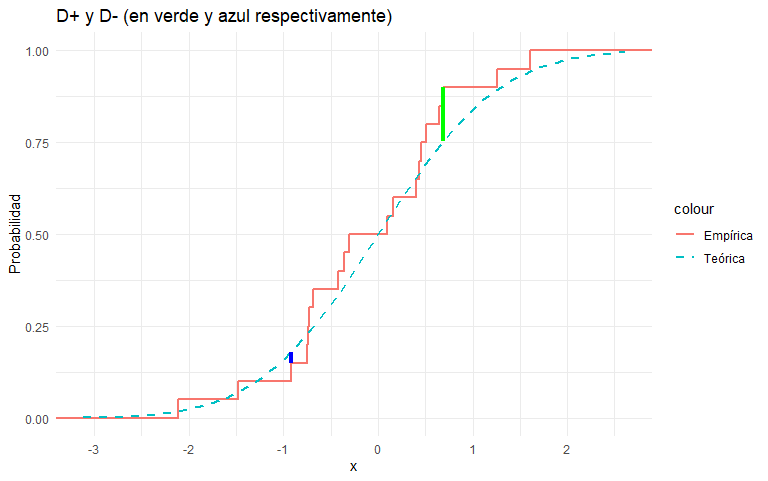
\includegraphics[width=\textwidth]{assets/Tema4/EjemploD.png}
    \caption{Visualización del estadísitico D+ y D-}
    \label{fig:Dplus_Dminus}
\end{figure}

Definimos los estadísticos de orden como $X_{(0)}=-\infty$ y $X_{(n)}=+\infty$, por lo tanto podemos definir $\widehat{F_n}(x)=\frac{i}{n} \quad \forall X_{(i)} \leq x < X_{(i+1)}$.

$D_n^+$ lo podemos ir calculando a trozos como:

\[
    D_n^+=sup_x(\widehat{F_n}(x)-F_0(x))
\]
    
Tomará un valor máximo unicamente en los extremos del intervalo $[X_{(i)},X_{(i+1)})$        
            
\[
    D_n^+=max_{1 \leq i \leq n}\left(\frac{i}{n}-F_0(x_{(i)})\right)
\]
Análogamente:
\[
    D_n^-=max_{1 \leq i \leq n}\left(F_0(x_{(i)})-\frac{i-1}{n}\right)
\]
$D_n^+,D_n^-$(por lo tanto $D_n$) dependen de las variables aleatorias.
\[
F_0(X_{(1)}),\dots,F_0(X_{(n)}) \sim U(0,1)
\]
Esto ocurre por la trasnformada integral de probabilidad, siempre y cuando las variables aleatorias sean continuas.

\subsubsection{Test de Kolmogorov-Smirnov para una hipótesis compuesta}

Lo anterior nos sirve para hipótesis simples. Sin embargo en la mayoría de los escenarios reales, tenemos hipótesis compuestas.
Por ejemplo, utlizar Kolmogorov-Smirnov en ANOVA.

Situación:
\[
H_0: F=F_0(\theta) \quad H_1:F \neq F_0(\theta)
\]
Lo haremos como siempre:
\begin{enumerate}
    \item Estimamos $\theta$ a partir de los datos(con el Estimador Máximo Verosimil).
    \item Se calcula el estadístico Kolmogorov-Smirnov como en el caso de la hipótesis simple:
    \[
        \widehat{D_n}=sup_x|\widehat{F_n}(x)-F(x)|
    \]
    Se rechaza $H_0$ con valores grandes de $\widehat{D_n}$ ($\widehat{D_n}>C$). 
    
    Es importante recalcar que $\widehat{D_n}$ no sigue la misma distribución que $D_n$.
    La distribución no es libre, depende de la familia que estemos evaluando.
\end{enumerate}

Tenemos tablas obtenidas por \href{https://es.wikipedia.org/wiki/Prueba_de_Lilliefors}{Lilliefors}
por simulación para la normal y para la exponencial.
Pasos a seguir:
\begin{enumerate}
    \item Se estiman los parámetros $\hat{\mu}$ y $\widehat{\lambda}$
    \item Se obtiene la muestra estandarizada $z_1,\dots,z_n$.
    \item Hacer el test ($H_0:F_0 \equiv N(0,1)$ en el caso normal y $H_0:F_0\equiv exp(1)$ en el caso exponencial).
    \item Se rechaza $H_0$ si $\widehat{D_n}>C$ para nivel $\alpha$. Se usan las tablas de \href{https://es.wikipedia.org/wiki/Prueba_de_Lilliefors}{Lilliefors}
    para definir $C_\alpha$.
\end{enumerate}

\textbf{Caso exponencial:}

\[
\begin{matrix}
    H_0:F \equiv exp(\lambda) \\
    H_1:F \not\equiv exp(\lambda)
\end{matrix}
\]
\[
    \widehat{\lambda}=\frac{1}{\bar{X}}, \quad z_i
    =\frac{X_i}{\bar{X}} \to z_i \sim exp(1)=\gamma(1,\lambda)
\]
El contraste es equivalente a:
\[
    H_0: X \sim \gamma\left(1,\frac{1}{\bar{X}}\right) \longleftrightarrow H_0:Z \sim \gamma(1,1)
\]

\vspace*{5mm}

\noindent Podrás descubrir más estadísticos en el campus virtual

\newpage
\section{Test de Shapiro-Wilk}
(Este test es más potente que el de Kolmogorov-Smirnov)

Mide como de bien se ajustan los datos a una distribución normal esperada. Se basa en combinación lineal de estadísticos ordenados. %Esto lo ha añadido en clase

\[
    W=\frac{\left(\sum_{i=1}^{n} a_i \cdot \chi_{(i)}\right)^2}{\sum_{i=1}^{n}(\chi_i-\bar{X})^2}
\]

donde

\begin{itemize}
    \item $\chi_{(i)} \longrightarrow$ estadístico de orden i.
    \item $a_i \longrightarrow$ coeficientes calculados a partir de los cuartiles esperados de una distribución normal estandar. 
\end{itemize}

\[
    (a_1,a_2,\dots,a_n)=\frac{m^T\cdot v^{-1}}{\sqrt{m^T \cdot V^{-1} \cdot V^{-1} \cdot m}}
\]

tal que

\begin{itemize}
    \item m=($m_{(1)},\dots,m_{(n)}$)
    \item V es la matriz de las covarianzas de $m_{(i)}$
\end{itemize}

El numerador nos indica como de bien se alinean los datos con la normalidad esperada. Si los datos son normales, el numerador será grande.
\section{Primer examen parcial}

\textbf{Ejercicio 1:}

Un artículo, producto de un tipo de componente mecánico que puede deteriorarse a dos velocidades distintas, depende de factores de fabricación no controlados.  
Se observa que el tiempo de vida ($X$) de cada componente sigue una mezcla de distribuciones exponenciales con las siguientes características:

\begin{itemize}
    \item Con probabilidad \(p\), el componente tiene un tiempo de vida \(X\) que sigue una distribución exponencial con parámetro \(\lambda_1\), lo cual corresponde a componentes con alta resistencia.
    \item Con probabilidad \(1-p\), el componente tiene un tiempo de vida \(X\) que sigue una distribución exponencial con parámetro \(\lambda_2\), lo cual corresponde a componentes con menor resistencia.
\end{itemize}

El fichero \texttt{Tiempos.RData} corresponde a un conjunto de observaciones independientes \(x_1, x_2, \dots \), que representan los tiempos de vida medidos en horas de varios componentes.

\begin{enumerate}
    \item Obtener el EMV y concretar su distribución asintótica para los parámetros del modelo que subyace a partir de estos datos.
    \textbf{Nota:} Planteadas las ecuaciones de verosimilitud, utilice la función \texttt{optim} para el cálculo del EMV.

    \[
    f(x, p, \lambda_1, \lambda_2) = p \cdot e^{-\lambda_1 x} + (1-p) \cdot e^{-\lambda_2 x}
    \]

    \[
    L(x, p, \lambda_1, \lambda_2) = \prod_{i=1}^{n} f(x_i, p, \lambda_1, \lambda_2) = \prod_{i=1}^{n} \left( p \cdot e^{-\lambda_1 x_i} + (1-p) \cdot e^{-\lambda_2 x_i} \right)
    \]

    \[
    \log L(x, p, \lambda_1, \lambda_2) = \sum_{i=1}^{n} \log f(x_i, p, \lambda_1, \lambda_2)
    \]

    \[
    \begin{pmatrix}
        \widehat{p} \\
        \widehat{\lambda}_1 \\
        \widehat{\lambda}_2
    \end{pmatrix}
    \sim
    N_3
    \left(
    \begin{pmatrix}
        p \\
        \lambda_1 \\
        \lambda_2
    \end{pmatrix},
    \text{Var}(\text{EMV})_{3 \times 3}
    \right)
    \]

    \item Obtener el IC de Wald con confianza aproximada de \(95\%\) para cada parámetro del modelo.

    \[
    \widehat{p} \pm \texttt{qnorm}(0.975) \cdot \sqrt{\text{Var}(\widehat{p})}
    \]

    \item Obtener el \textit{p-valor} basado en el estadístico de Wald para contrastar la hipótesis \(H_0: \lambda_1 = 0.5\) vs. \(H_a: \lambda_1 \neq 0.5\).

    \[
    W = \frac{(\widehat{\lambda}_1 - 0.5)^2}{\text{Var}(\widehat{\lambda}_1)} \sim \chi^2_1
    \]

    \item Obtener el \textit{p-valor} basado en el estadístico de RV para contrastar la hipótesis \(H_0: \lambda_1 = 0.5\) vs. \(H_a: \lambda_1 \neq 0.5\).

    \[
    Q_L = 2 \cdot \left[ \log L(\widehat{p}, \widehat{\lambda}_1, \widehat{\lambda}_2, x) - \sup_{p, \lambda_2} \log L(p, \lambda_1 = 0.5, \lambda_2, x) \right] \sim \chi^2_1
    \]

\end{enumerate}


\newpage

% ------------------------------------------------------------------------------
% Reference and Cited Works
% ------------------------------------------------------------------------------

\begin{thebibliography}{9}
    \bibitem{diapos1}
    Juan Camilo Yepes Borrero, \\ \textit{Apuntes Manuscritos Tema 4}. \\ Universidad de Valladolid 2024.
    \bibitem{diapos2}
    Yolanda Larriba González, \\ \textit{Apuntes INFE2 Tema 4}. \\ Universidad de Valladolid 2023.
\end{thebibliography}

% ------------------------------------------------------------------------------

\end{document}
